\documentclass{article}
\usepackage{t1enc}
\usepackage{amsmath, amssymb, amsfonts}
\usepackage{fullpage}
\usepackage{hyperref}
\usepackage{dirtytalk}
\usepackage{graphicx}
\usepackage{enumerate}
\frenchspacing
\usepackage[latin2]{inputenc}
\usepackage{tikz}
\usepackage{scalefnt}
\usetikzlibrary{shapes,shapes.geometric,arrows,fit,calc,positioning,automata,}
\tikzset{dot/.style={circle,fill=#1,inner sep=0,minimum size=4pt}}

\newtheorem{tetel}{T�tel}[section]
\newtheorem{pl}[tetel]{P�lda}
\newcommand{\Mod}[1]{\ (\text{mod}\ #1)}

\title{Datamining project: Taxi destination prediction}
\author{B�res Ferenc}

\begin{document}

\maketitle

\section{Introduction}

This project is related to the Discovery Challange of the \href{http://www.geolink.pt/ecmlpkdd2015-challenge/}{ECML 2015} conference. The original contest was announced on \href{https://www.kaggle.com/c/pkdd-15-predict-taxi-service-trajectory-i}{Kaggle}. I chose this dataset because I mainly work on projects related to classification, but this task is a regression problem as I have to predict the destinations of taxi routes.

\subsection{ECML Challange 2015}

In the original contest there were two tasks:

\begin{enumerate}
\item Taxi trajectory prediction
\item Taxi trip time prediction
\end{enumerate}

The main motivation behind these tasks can be read on the Kaggle site:

\vspace{12pt}

\say{To improve the efficiency of electronic taxi dispatching systems it is important to be able to predict the final destination of a taxi while it is in service. Particularly during periods of high demand, there is often a taxi whose current ride will end near or exactly at a requested pick up location from a new rider. If a dispatcher knew approximately where their taxi drivers would be ending their current rides, they would be able to identify which taxi to assign to each pickup request.}

\vspace{12pt}

\subsection{Evaluation metric}

The evaluation metric for this competition is the \emph{Mean Haversine Distance}. The Haversine Distance is commonly used in navigation. It measures distances between two points on a sphere based on their latitude and longitude.

The Harvesine Distance between the two locations can be computed as follows

\begin{equation}
a=\sin^{2}{\frac{\phi_{1}-\phi_{2}}{2}}+\cos{\phi_1}\cos{\phi_2}\sin^{2}{\frac{\lambda_{1}-\lambda_{2}}{2}}
\end{equation}
\begin{equation}
d = 2 \cdot r \cdot atan \sqrt{\frac{a}{1-a}}
\end{equation}

where $\phi$ is the latitude, $\lambda$ is the longitude, $d$ is the distance between two points, and $r$ is the sphere's radius, 

In our case, it should be replaced by the Earth's radius in the desired metric (e.g., $6371$ kilometers).

\vspace{12pt}

In the ECML contest the winner models had performance approximately $2$ km which you can see on Figure~\ref{fig:priv_kaggle}.

\begin{figure}
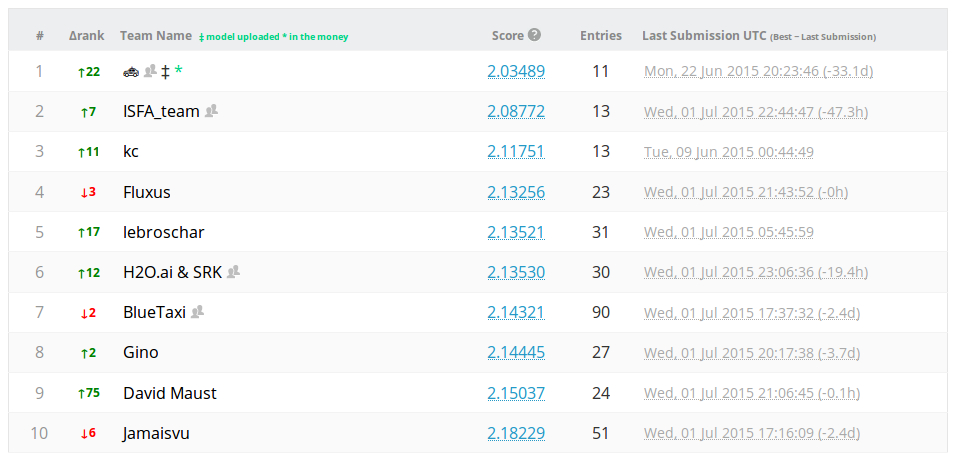
\includegraphics[scale=0.5]{img/private_board.png}
\caption{Private leaderboard of the original challange. The score is the mean Haversine distance in kilometres.}
\label{fig:priv_kaggle}
\end{figure}

\section{Data preparation}

The original dataset contains information about taxi rides in Porto, the capital of Portugal. In the challange there is a \emph{training set} and a \emph{testing set} provided for the participants. In the training set the full route trajectory is available but for the testing set only the first few locations.

\subsection{Restrictions}

Due to the size of the original training set (1710670 records) I made some restrictions. I only used the first 50000 records from the original training set to build models. From the testing set I excluded 6 outlier records due to the fact that in this project I only used $\approx3\%$ of the original training data.

\begin{center}
\begin{tabular}{ |l|c|c| } 
\hline
 & \textbf{Train} & \textbf{Test} \\ 
\hline
 \textbf{Average trajectory length} & 45.85 & 43.12 \\ 
\hline
\textbf{Number of records} & 50000 & 325 \\ 
\hline
\end{tabular}
\end{center}

\subsection{Feature engineering}

\subsubsection{Location precision}

In the original data latitude and longitude coordinates are given with $10^{-6}$ precision. In order to use GPS information in features I chose to decrease this precision. Before generating new features I rounded latitude values to $10^{-3}$ (approx. $1$km) precision and longitude values to $10^{-2} $(approx. $100$m) precision (see Figure~\ref{fig:gps_prec}). The reason why I chose to use more precision for the latitude was the localization of Porto. The city is along the coast of the atlantic ocean so it has great vertical expansion so latitude is more important than longitude. During model evaluation I use the original destination GPS coordinates, always with $10^{-6}$ precision. The table below contains the rounded features for latitude. Similar features are generated for the longitude as well.

\begin{center}
\begin{tabular}{ |l|l| } 
\hline
 \textbf{Name} & \textbf{Description} \\ 
\hline
DEPARTURE\_LAT & The rounded departure latitude coordinate \\ 
\hline
DESTINATION\_LAT & The rounded destination latitude coordinate \\
\hline 
\end{tabular}
\end{center}

\begin{figure}
\centering
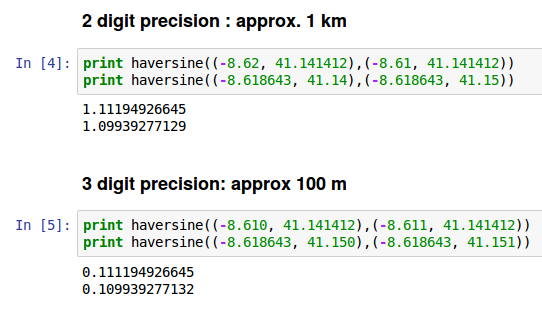
\includegraphics[scale=0.5]{img/gps_precision.png}
\caption{GPS location precision in distance for latitude and longitude}
\label{fig:gps_prec}
\end{figure}

\subsubsection{Aggregation based features}

I summarize each taxi route by aggregation based features. In the following table you can find the list of generated features related to trajectories.

\begin{center}
\begin{tabular}{ |l|l| } 
\hline
 \textbf{Name} & \textbf{Description} \\ 
\hline
TRIP\_SIZE & The number of locations in a trajectory \\ 
\hline
TRIP\_LAT\_UNIQUE & The number of unique latitude values in a trajectory \\ 
\hline
TRIP\_LAT\_UNIQUE\_RATIO & TRIP\_LAT\_UNIQUE / TRIP\_SIZE \\ 
\hline
TRIP\_LAT\_MIN & The minimum latitude value in a trajectory \\ 
\hline
TRIP\_LAT\_MAX & The maximum latitude value in a trajectory \\ 
\hline
TRIP\_LAT\_MEAN & The mean of latitude values in a trajectory \\ 
\hline
TRIP\_LAT\_MEDIAN & The median of latitude values in a trajectory \\ 
\hline
TRIP\_LAT\_STD & The standard deviation of latitude values in a trajectory \\ 
\hline
TRIP\_LAT\_MIN\_DIFF & DEPARTURE\_LAT - TRIP\_LAT\_MIN \\ 
\hline
TRIP\_LAT\_MAX\_DIFF & DEPARTURE\_LAT - TRIP\_LAT\_MAX \\ 
\hline
TRIP\_LAT\_MEAN\_DIFF & DEPARTURE\_LAT - TRIP\_LAT\_MEAN \\ 
\hline
TRIP\_LAT\_MEDIAN\_DIFF & DEPARTURE\_LAT - TRIP\_LAT\_MEDIAN \\ 
\hline
\end{tabular}
\end{center}

Similar features are generated for the longitude as well.

\subsubsection{Time based features}

Originally, only TIMESTAMP is given. From this I generate the following features: 

\begin{center}
\begin{tabular}{ |l|l| } 
\hline
 \textbf{Name} & \textbf{Description} \\ 
\hline
DAY\_OF\_WEEK & Index of the day of the week \\ 
\hline
TIME\_OF\_DAY & HOUR // 6 (integer division) \\
\hline 
\end{tabular}
\end{center}

%\subsubsection{Onehot Encoding}

\section{Model selection}

In this project I propose a two-phase model setting for solving the problem of taxi route destination prediction. The first step is a GBT regression model which predicts approximate destination using only rounded GPS coordinates. Then based on the predictions of the GBT, I specify the final destination with $k$-NN models. I also suggest a baseline model which performs well but it is rather theoretical than practical.

\subsection{Gradient Boosted Trees for regression}

I trained two regression models. One for the latitude coordinate and another for the longitude coordinate. Both models were trained only for the rounded destination coordinates (DESTINATION\_LAT, DESTINATION\_LNG) as I only would like to get approximate locations from GBT. I experimented with different model parameters, from which 40 tree and 5 depth seemed to be the most promising. You can see the mean Haversine distance for the testing set regarding GBT model parameters on the table below.

\begin{center}
\begin{tabular}{ |l|c|c|c|c|c| } 
\hline
 \textbf{Number of Trees} & 50 & 40 & 30 & 30 & 30 \\ 
\hline
 \textbf{Maximum Depth} & 5 & 5 & 5 & 4 & 3 \\ 
\hline
\textbf{Mean Haversine} & 0.708 & \textbf{0.726} & 0.791 & 0.847 & 0.938 \\
\hline 
\end{tabular}
\end{center}

Figure~\ref{fig:gbt_imp} shows feature importances of the GBT models using 40 tree with 5 depth each.

\begin{figure}[h!]
\centering
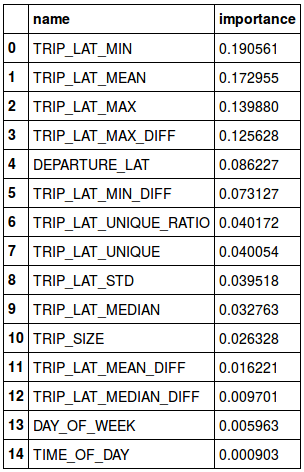
\includegraphics[scale=0.6]{img/lat_gbt.png}
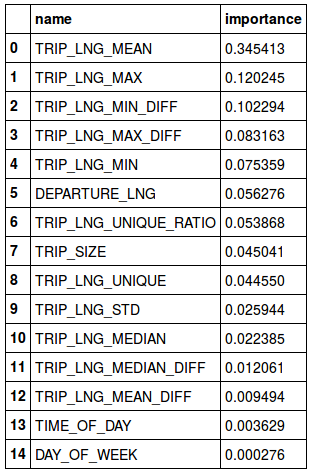
\includegraphics[scale=0.6]{img/lng_gbt.png}
\caption{\textbf{Left:} feature importance of the latitude GBT model, \textbf{Right:} feature importance of the longitude GBT model.}
\label{fig:gbt_imp}
\end{figure}


\subsection{Baseline mean predictor}

As GBT models were trained for only approximate destination coordinates, they cannot achieve such a good performance. In order to improve the model quality I compute the mean destination in each rounded cell only for the training set. Then my final prediction for a test record $r$ is the following:

\begin{enumerate}
\item Predict an approximate destination for route $r$ with GBT $(x_{gbt},y_{gbt})$.
\item Identify the location cell $C_{i}$ that contains $(x_{gbt},y_{gbt})$.
\item Predict the mean of destinations of the training set in $C_{i}$ for the route $r$ as destination.
\end{enumerate}

Although this modification improves the model significantly, there is a major disadvantage. In a given location cell a specific location, the mean destination, is predicted for all routes. That is why I chose this model as a baseline because I think it is rather a theoretical model. In a real application we would like different locations to be assigned for different routes. 

\subsection{Specifying destinations with $k$-NN}

In order to predict more diverse destinations I use k-NN models. First, I train $k$-NN models for each location cell in the training set. After the models were trained I predict final destination in the following way:

\begin{enumerate}
\item Predict an approximate destination for route $r$ with GBT $(x_{gbt},y_{gbt})$.
\item Identify the location cell $C_{i}$ that contains $(x_{gbt},y_{gbt})$.
\item Predict the mean of the $k$ nearest neighbors, with the $k$-NN model trained on cell $C_{i}$, for the route $r$ as destination. In case there are less than $k$ records in $C_{i}$ then the mean of those locations is proposed.
\end{enumerate}

$k$-NN models use only a subset of the generated features (DEPARTURE\_LAT, TRIP\_LAT\_MEAN, TRIP\_LAT\_MIN, TRIP\_LAT\_MAX, TRIP\_LAT\_MEDIAN, DEPARTURE\_LNG, TRIP\_LNG\_MEAN, TRIP\_LNG\_MIN, TRIP\_LNG\_MAX, TRIP\_LNG\_MEDIAN, DESTINATION\_LAT\_FULL, DESTINATION\_LNG\_FULL). These features were selected based on their feature importance in GBT models. At first I wanted to define a custome weighted distance for $k$-NN but scikit learn could not integrate it. But the results are still good using only euclidean distance.

\section{Results}

Unfortunately, my results are hard to compare with results from the private leaderboard due to two reasons:

\begin{itemize}
\item In the original contest the leaderboard (public or private) are based only on 50-50\% of the testing set. While I use the full testing set for evaluation
\item From the testing set I excluded 6 outlier destinations.
\end{itemize}

On the other hand I could achieve similar results with the $k$-NN based model to the baseline model. It is good because the baseline model has good performance but it is impractical. The following table show the mean Haversine ditance for the models examined in this project.

\begin{center}
\begin{tabular}{ |l|l|l|l| } 
\hline
 & \textbf{GBT (40 tree, 5 depth)} & \textbf{Mean predictor} & \textbf{$k$-NN predictor} \\ 
\hline
 \textbf{Mean Haversine} & 0.726317 & 0.172401 & \textbf{0.173984} \\ 
\hline
\end{tabular}
\end{center}

We can see that the mean predictor and the $k$-NN predictor have similar performances, and they outperform GBT model. But altogether GBT was good enough to predict and approximation location cell for the route destination. Figure~\ref{fig:result_pred} shows that the predictions for the $k$-NN model are indeed more diverse than for the baseline which is a big advantage in this application.

\begin{figure}
\centering
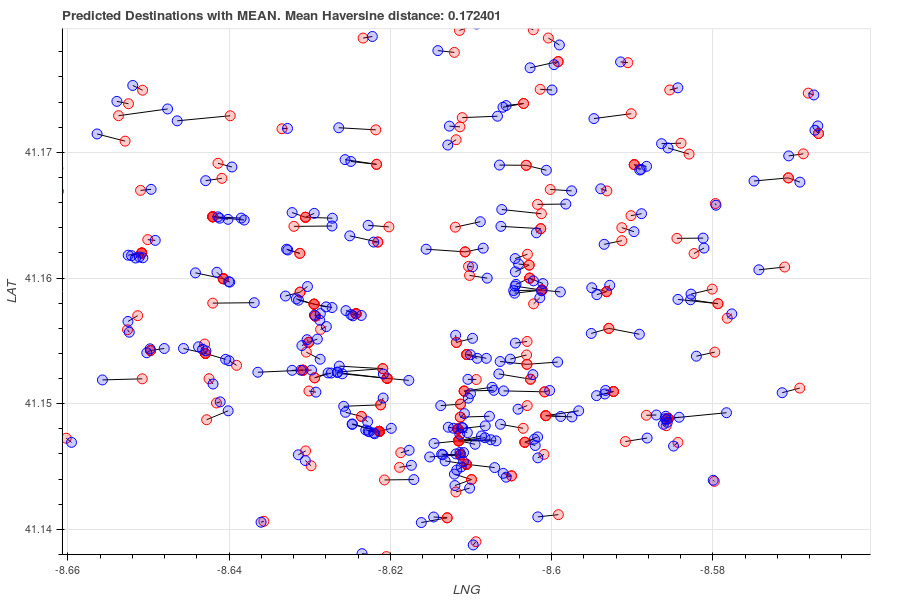
\includegraphics[scale=0.45]{img/mean_pred.png}
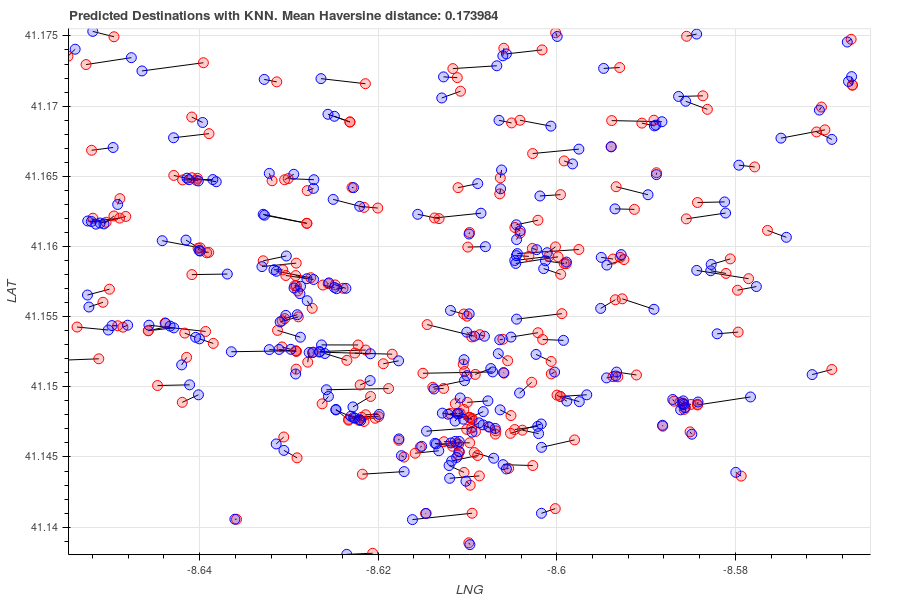
\includegraphics[scale=0.45]{img/knn_pred.png}
\caption{Predictions of the baseline (top) and $k$-NN predictor (bottom). models in the city centre of Porto. Blue circles are the real destination, while red ones are the predictions. Black lines represent the error.}
\label{fig:result_pred}
\end{figure}

\section{Implementation}

In this project I used \emph{Python} (pandas, numpy, sklearn). The data preparation, model selection and final destination prediction are implemented in different \emph{Jupyter} notebooks.

\vspace{12pt}

The notebooks of this project are organized into a \textbf{Datawand} pipeline. \emph{Datawand} is my custom Jupyter notebook manager framework, not yet publically available. With \emph{Datawand} I can schedule and parametrize notebooks based on custom configuration. On Figure~\ref{fig:luigi_dep} you can see the dependencies between different tasks of the pipeline.

\begin{figure}[h!]
\centering
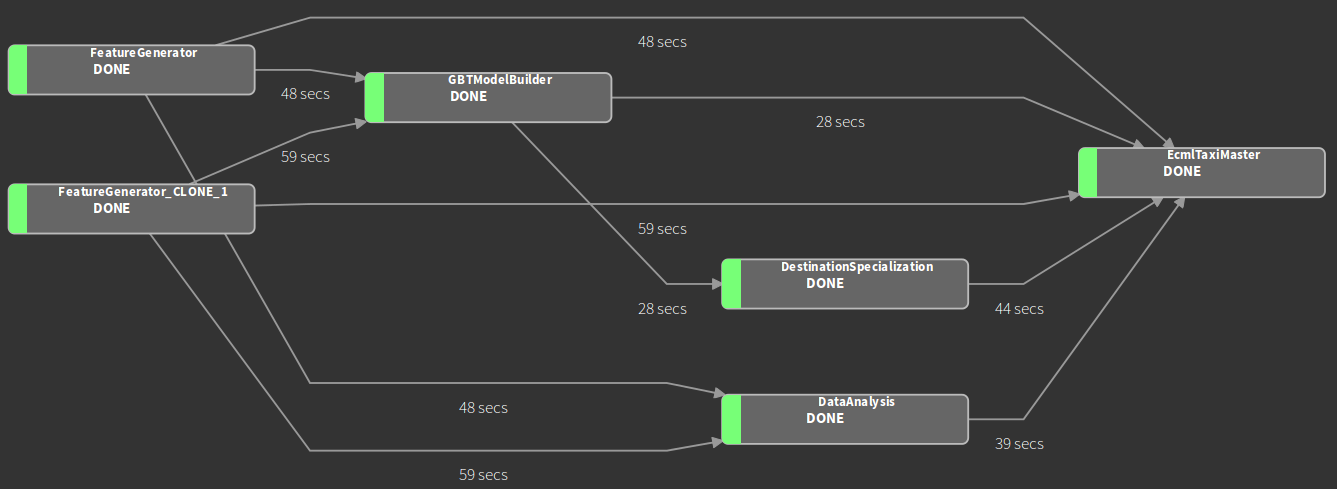
\includegraphics[scale=0.3]{img/luigi_plan.png}
\caption{Pipeline dependencies}
\label{fig:luigi_dep}
\end{figure}

\section{Summary}

In this project I solved the problem of taxi route destination prediction. I propose a two-phase modeling framework. The first model is a GBT which use rounded GPS locations. In the second phase I use several $2$-NN models to predict the final destination based on the output of the GBT model. With this setting I could achieve approximately $173$ meter mean error for Haversine distance.  

\end{document}